\documentclass[11pt,letterpaper]{article}
\usepackage{../acl2015}
\usepackage{times}
\usepackage{latexsym}
% \setlength\titlebox{7.5cm}    % Expanding the titlebox

%%% Custom additions %%%
\usepackage{url}
\usepackage[leqno, fleqn]{amsmath}
\usepackage{amssymb}
\usepackage{qtree}
\usepackage{graphicx}
\usepackage{booktabs}
\usepackage{multirow}
\usepackage{colortbl}
\usepackage{caption}
\usepackage{subcaption}
\usepackage{color}
\usepackage{xcolor}
\usepackage{tikz}
\usepackage{tikz-qtree}
\usepackage{ifthen}
\usepackage{framed}


\newcommand\todo[1]{\textcolor{blue}{\textbf{TODO:} #1}}
\newcommand\result[1]{\textcolor{red}{\textbf{RESULT NEEDED:} #1}}
\newcommand\question[1]{\textcolor{orange}{\textbf{OPEN QUESTION:} #1}}

\newcount\colveccount
\newcommand*\colvec[1]{
        \global\colveccount#1
        \begin{bmatrix}
        \colvecnext
}
\def\colvecnext#1{
        #1
        \global\advance\colveccount-1
        \ifnum\colveccount>0
                \\
                \expandafter\colvecnext
        \else
                \end{bmatrix}
        \fi
}

\newcommand{\nateq}{\equiv}
\newcommand{\natind}{\mathbin{\#}}
\newcommand{\natneg}{\mathbin{^{\wedge}}}
\newcommand{\natfor}{\sqsubset}
\newcommand{\natrev}{\sqsupset}
\newcommand{\natalt}{\mathbin{|}}
\newcommand{\natcov}{\mathbin{\smallsmile}}

\newcommand{\plneg}{\mathop{\textit{not}}}
\newcommand{\pland}{\mathbin{\textit{and}}}
\newcommand{\plor}{\mathbin{\textit{or}}}

\newcommand{\shift}{\textsc{shift}}
\newcommand{\reduce}{\textsc{reduce}}

% Strikeout
\newlength{\howlong}\newcommand{\strikeout}[1]{\settowidth{\howlong}{#1}#1\unitlength0.5ex%
\begin{picture}(0,0)\put(0,1){\line(-1,0){\howlong\divide\unitlength}}\end{picture}}

\newcommand{\True}{\texttt{T}}
\newcommand{\False}{\texttt{F}}
\usepackage{stmaryrd}
\newcommand{\sem}[1]{\ensuremath{\llbracket#1\rrbracket}}

\newcommand{\mynote}[1]{{\color{blue}#1}}
\newcommand{\tbchecked}[1]{{\color{red}#1}}

\usepackage{gb4e}
\noautomath
 
\def\ii#1{\textit{#1}}
\newcommand{\word}[1]{\emph{#1}}
\newcommand{\fulllabel}[2]{\b{#1}\newline\textsc{#2}}


%%%%%%%%%%%%%%%%%%%%%%%%%%%%%%%%%%%%%%%%%%%%%%%%%%%%%%%%%%%%%%%%%%%%%%
%%%%% Code to simulate natbib's citealt, which prints citations with
%%%%% no parentheses:

\makeatletter
\def\citealt{\def\citename##1{{\frenchspacing##1} }\@internalcitec}
\def\@citexc[#1]#2{\if@filesw\immediate\write\@auxout{\string\citation{#2}}\fi
  \def\@citea{}\@citealt{\@for\@citeb:=#2\do
    {\@citea\def\@citea{;\penalty\@m\ }\@ifundefined
       {b@\@citeb}{{\bf ?}\@warning
       {Citation `\@citeb' on page \thepage \space undefined}}%
{\csname b@\@citeb\endcsname}}}{#1}}
\def\@internalcitec{\@ifnextchar [{\@tempswatrue\@citexc}{\@tempswafalse\@citexc[]}}
\def\@citealt#1#2{{#1\if@tempswa, #2\fi}}
\makeatother

%%%%%%%%%%%%%%%%%%%%%%%%%%%%%%%%%%%%%%%%%%%%%%%%%%%%%%%%%%%%%%%%%%%%%

\title{A unified model for parsing and sentence understanding} 

%    \author{
%    Samuel R.\ Bowman$^{1,2,5,}$\thanks{The first two authors contributed equally.} \\
%    \texttt{\small sbowman@stanford.edu} \\
%    \And
%    Jon Gauthier$^{2,3,5,*}$ \\
%    \texttt{\small jgauthie@stanford.edu} \\
%    \And
%    Abhinav Rastogi$^{4,5}$ \\
%    \texttt{\small arastogi@stanford.edu} \\
%    \AND
%    Raghav Gupta$^{6}$ \\
%    \texttt{\small rgupta93@stanford.edu} \\
%    \And
%    Christopher D.\ Manning$^{1,2,5,6}$\\
%    \texttt{\small manning@stanford.edu}\\
%    \And
%    Christopher Potts$^{1}$\\
%    \texttt{\small cgpotts@stanford.edu}
%    \AND\\[-3ex]
%    {$^{1}$Stanford Linguistics\quad
%    $^{2}$Stanford NLP Group\quad
%    $^{3}$Stanford Symbolic Systems}\\
%    {$^{4}$Stanford Electrical Engineering\quad
%    $^{5}$Stanford AI Lab\quad
%    $^{6}$Stanford Computer Science}
%    }

\date{}

\makeatletter
\newcommand{\@BIBLABEL}{\@emptybiblabel}
\newcommand{\@emptybiblabel}[1]{}
\definecolor{black}{rgb}{0,0,0}
\makeatother
\usepackage[breaklinks, colorlinks, linkcolor=black, urlcolor=black, citecolor=black]{hyperref}

\def\t#1{#1}
\def\b#1{\t{\textbf{#1}}}
\def\colspaceS{2.25mm}
\def\colspaceM{4.0mm}
\def\colspaceL{4.25mm}

\begin{document}
\maketitle
\begin{abstract}

Tree-structured neural networks integrate valuable syntactic parse information into the process of interpreting sentence meaning, but suffer two key technical problems. They can only operate on parsed sentences and do not directly support batched computation, making them slow and unwieldy for large-scale NLP tasks. We address these issues by introducing the Parser-Interpreter Neural Network (PINN), which simulates tree-structured sentence interpretation within the sequential structure of a transition-based neural parser. This model  supports batched computation, and its integrated parser allows it to operate on unparsed data with nearly no loss of accuracy. We evaluate it on the Stanford NLI entailment task, show that it outperforms other sentence encoding models, and show that it can be integrated effectively with soft attention for sentence pair tasks like entailment for further gains in performance.
\todo{[SB] Revise according to comments.}
\end{abstract}

\question{Parser--Interpreter or Parser-Interpreter (hyphen or en-dash)?}

\section{Introduction}

%!TEX root = paper.tex

\begin{figure}[t]

\begin{subfigure}[t]{\columnwidth}
 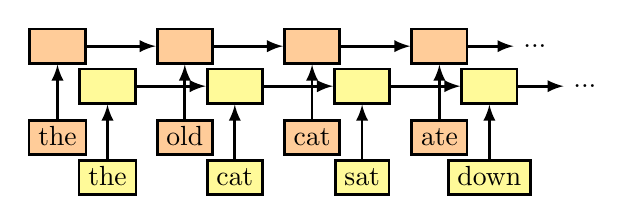
\begin{tikzpicture}
    \tikzstyle{word}=[fill=yellow!40,text height=2mm,line width=1pt,draw=black]    
    \tikzstyle{nonleaf}=[fill=yellow!40,text height=2mm,line width=1pt,draw=black] 
    \tikzstyle{alt}=[fill=orange!40]
    \pgfsetarrowsend{latex}
    \tikzstyle{fwd} = [draw=black, line width=1pt]
   
    \def\dx{23pt}
    \def\dy{11pt}
    \def\sy{7*\dy}
    \def\oxb{5.5*\dx}
    \def\by{1*\dy}
    \def\ox{0*\oxb}


    \begin{scope}[shift={(0in,0in)}, frontier/.style={distance from root=60pt}]
    
    \node[word,alt]  (w1) at (\ox+-3*\dx,\by+0*\dy) {the};
    \node[word,alt]  (w2) at (\ox+-1*\dx,\by+0*\dy) {old};
    \node[word,alt]  (w3) at (\ox+1*\dx,\by+0*\dy) {cat};
    \node[word,alt]  (w4) at (\ox+3*\dx,\by+0*\dy) {ate};

    \node[word,alt]  (n1) at (\ox+-3*\dx,\by+3*\dy) {~~~~~};
    \node[word,alt]  (n2) at (\ox+-1*\dx,\by+3*\dy) {~~~~~};
    \node[word,alt]  (n3) at (\ox+1*\dx,\by+3*\dy) {~~~~~};
    \node[word,alt]  (n4) at (\ox+3*\dx,\by+3*\dy) {~~~~~};
    \node[]  (n5) at (\ox+4.5*\dx,\by+3*\dy) {...};

   \draw [fwd] (w1) -- (n1);
   \draw [fwd] (w2) -- (n2);
   \draw [fwd] (w3) -- (n3);
   \draw [fwd] (w4) -- (n4);

   \draw [fwd] (n1) -- (n2);
   \draw [fwd] (n2) -- (n3);
   \draw [fwd] (n3) -- (n4);
   \draw [fwd] (n4) -- (n5);


    \end{scope}

    \begin{scope}[shift={(0.25in,-0.2in)}, frontier/.style={distance from root=60pt}]
    
    \node[word]  (w1) at (\ox+-3*\dx,\by+0*\dy) {the};
    \node[word]  (w2) at (\ox+-1*\dx,\by+0*\dy) {cat};
    \node[word]  (w3) at (\ox+1*\dx,\by+0*\dy) {sat};
    \node[word]  (w4) at (\ox+3*\dx,\by+0*\dy) {down};

    \node[word]  (n1) at (\ox+-3*\dx,\by+3*\dy) {~~~~~};
    \node[word]  (n2) at (\ox+-1*\dx,\by+3*\dy) {~~~~~};
    \node[word]  (n3) at (\ox+1*\dx,\by+3*\dy) {~~~~~};
    \node[word]  (n4) at (\ox+3*\dx,\by+3*\dy) {~~~~~};
    \node[]  (n5) at (\ox+4.5*\dx,\by+3*\dy) {...};


   \draw [fwd] (w1) -- (n1);
   \draw [fwd] (w2) -- (n2);
   \draw [fwd] (w3) -- (n3);
   \draw [fwd] (w4) -- (n4);

   \draw [fwd] (n1) -- (n2);
   \draw [fwd] (n2) -- (n3);
   \draw [fwd] (n3) -- (n4);
   \draw [fwd] (n4) -- (n5);

    \end{scope}

\end{tikzpicture}


\caption{\label{fig:batching:good}A conventional sequence-based RNN, instantiated for two sentences.}
\end{subfigure}

\vspace{2em}

\begin{subfigure}[t]{\columnwidth}
\begin{center}
 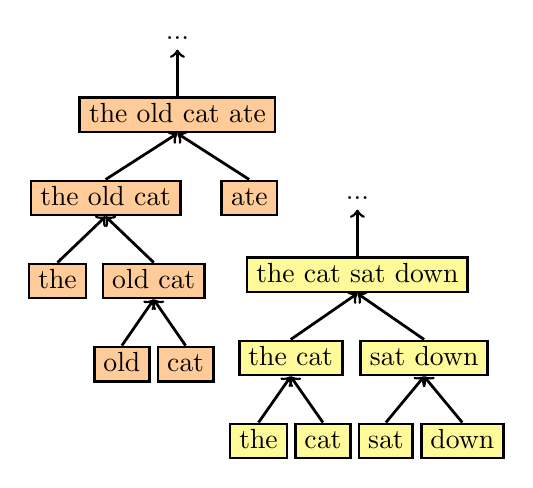
\begin{tikzpicture}
    \tikzstyle{word}=[fill=yellow!40,text height=2mm,line width=1pt,draw=black]    
    \tikzstyle{nonleaf}=[fill=yellow!40,text height=2mm,line width=1pt,draw=black]
    \tikzstyle{alt}=[fill=orange!40]    
    \pgfsetarrowsend{latex}
    \tikzset{edge from parent/.append style={<-, line width=1pt}}   

    \begin{scope}[shift={(0in,0in)}]

    \Tree [.\node[](root){...}; [.\node[nonleaf,alt](2thekittenate){the old cat ate}; [.\node[nonleaf,alt](2thekitten){the old cat}; \node[word,alt](2the){the}; [.\node[nonleaf,alt](2bigkitten){old cat}; \node[word,alt](2kitten){old}; \node[word,alt](2kitten){cat}; ] ] \node[word,alt](2ate){ate}; ] ]

    \end{scope}


    \begin{scope}[shift={(0.9in,-0.8in)}]

    \Tree [.\node[](root){...}; [.\node[nonleaf](1thecatsatdown){the cat sat down}; [.\node[nonleaf](1thecat){the cat}; \node[word](1the){the}; \node[word](1cat){cat}; ] [.\node[nonleaf](1satdown){sat down}; \node[word](1sat){sat}; \node[word](1down){down}; ] ] ]

    \end{scope}

\end{tikzpicture}
\end{center}

\caption{\label{fig:batching:bad}A conventional TreeRNN, instantiated for two sentences.}
\end{subfigure}

\caption{An illustration of two standard designs for sentence encoders. Note that the TreeRNN, unlike the sequence-based RNN, requires a substantially different connection structure for each sentence.}
\end{figure}


\begin{itemize}

\item Brief history of TreeRNNs
\begin{itemize}
\item Lx theory suggests should be better than comparable sequence models via compositionality \cite{Partee84,Janssen97}.
\item In practice, results mixed but positive. \citealt{tai2015improved} shows dramatic gains on sentiment analysis using tree-structured models over sequence models. \citealt{li2015tree} shows mixed results. Both of these evaluations are limited to small datasets with only hundreds or thousands of training examples.
\item Larger evaluations have been impossible due to issues of computational efficiency. One aim of this paper is to mitigate these issues to make larger-scale experiments possible.
\item Note, though, that while tree structure can be seen as a bias, simply adding more data within reason may not be enough to get a sequence model to learn without that bias \citealt{bowman2015trees}.
\end{itemize}

\item Speed issues
\begin{itemize}
\item Efficient batched computation is a crucial enabling technology in allowing NNs to be used on large datasets. Since NNs require large datasets to be able to model complex problems like language understanding, this is crucial in NLP.
\item Tree structured neural networks can't be batched. As the schematic in Figure~\ref{fig:batching:bad} indicates, different sentences are assigned different trees, and there is no straightforward way of aligning these trees to synchronize computation in the conventional style of implementation.
\item In addition, the requirement of an external parser complicated pipeline-building, and slows down inference. This is not necessarily a practical limitation, since modern parsers can assign reasonably high quality parses in so little time as to not dramatically impact the performance characteristics of our model \todo{[SB,JG,CM] How fast are fast constit parsers?}.

\end{itemize}

\item Our model
\begin{itemize}
\item In this paper, we present the Parser--Interpreter NN (PINN) 

\end{itemize}

\item Attention issues
\begin{itemize}
\item The technique of soft attention has proven to be exceptionally effective as a way of training neural network models for tasks like translation \cite{bahdanau2014neural,luong-pham-manning:2015:EMNLP} and natural language inference \cite{rocktaschel2015reasoning}.
\item This paper proposes two complementary extensions of the idea of attention to tree-structured models:
\begin{itemize}
\item Constituent-by-constituent attention, in which each node in the tree of one sentence is given a soft alignment to some node or nodes in a second sentence.
\item The mTreeLSTM, which uses a third tree structured model to accumulate information about the alignment between two sentences into a single feature vector. This builds on the notion of a matching LSTM or mLSTM from \citealt{DBLP:journals/corr/WangJ15b}.
\end{itemize}
\end{itemize}

\item Outline of the paper
\begin{itemize}
\item Propose a model
\item Show how the model can be used for NLI
\item Show how attention can be used on the NLI model
\item Experiments and discussion
\end{itemize}

\end{itemize}

\section{The transition-based sentence model}

\subsection{Intuition: Transition-based parsing}

The PINN is based on a formalism adapted from transition-based parsing (\question{What's a good classic citation for this?}).

\todo{[SB, JG] Brief into to transition-based parsing.}

\vspace{10em}

\subsection{The model}

The PINN, which is shown in Figure~\ref{fig:model:0}, takes the form of a transition-based parser, but it is designed to produce sentence representations given parse structures, rather than producing parse structures as its output, leading to the following differences: \todo{[SB] Swap in Model 1 fig.}
\begin{itemize}
\item The model takes a sequence of transitions (\shift s or \reduce s) as input, rather than incorporating a decision function which chooses which transition to perform at each step.
\item The intermediate representations in the parser, including the representations of the tree structures on the stack, are vectors of a fixed length.
\item The \reduce~operation, which combines two trees or tree nodes on the stack into a single larger tree, is represented using a parametric neural network layer function (in particular, a TreeLSTM layer, after \citealt{tai2015improved}).
\item The intermediate states of the stack and buffer during parsing are stored during training. This makes it possible to learn the parameters of the composition function and the input word representations that are fed into the buffer using backpropagation on an objective function that depends on the final sentence representation that emerges at the head of the stack.
\item A novel tracking LSTM component is added to improve the model's ability to efficiently track the context in which each step is being performed.
\item A variant, PINN-GT uses ground truth parse information at training and test time, and omits the prediction layer.
\end{itemize}

%!TEX root = hard_stack_paper/paper.tex


\begin{figure*}[t]

\begin{subfigure}[t]{\textwidth}
\centering
\scalebox{0.6}{
 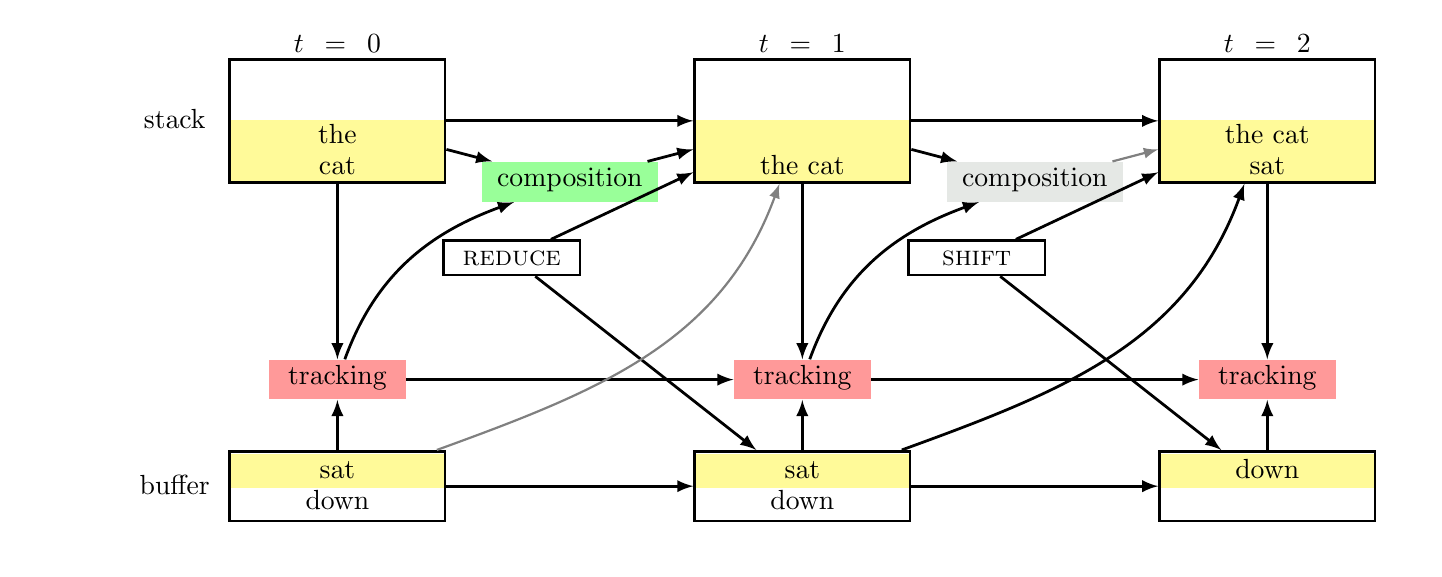
\begin{tikzpicture}
    \def\dx{21pt}
    \def\dy{11pt}
    \def\sy{13*\dy}
    \def\oxb{8*\dx}
    \def\by{1*\dy}
    \def\ox{0*\oxb}

    \tikzstyle{label}=[text width=35mm,align=center,text height=2mm]    
    \tikzstyle{word}=[text width=35mm,align=center,text height=2mm]    
    \tikzstyle{tracker}=[fill=red!40,text width=15mm,align=center,text height=2mm]
    \tikzstyle{softmax}=[fill=blue!40,text width=15mm,align=center,text height=2mm]
    \tikzstyle{comp}=[fill=green!40,text width=20mm,align=center,text height=2mm]
    \tikzstyle{compoff}=[fill=green!10!black!10,text width=20mm,align=center,text height=2mm]
    \tikzstyle{result}=[line width=1pt,draw=black,text width=15mm,align=center,text height=2mm]    
    \tikzstyle{sbox}=[line width=1pt,draw=black,text width=25mm,align=center,text height=13.3mm]
    \tikzstyle{bbox}=[line width=1pt,draw=black,text width=25mm,align=center,text height=6.5mm]
    \tikzstyle{focus1}=[fill=yellow!40,text width=25mm,align=center,text height=2mm]
    \tikzstyle{focus2}=[fill=yellow!40,text width=25mm,align=center,text height=5.5mm]

    \node[label]  (sl) at (\ox-0.35*\oxb+0*\dx,\by+0.5*\dy) {buffer};

    \node[label]  (1l) at (\ox+0*\dx,\sy+3*\dy) {$t=0$};

    \node[focus1] (0bb) at  (\ox+0*\dx,2*\dy) {};
    \node[word]  (0b3) at (\ox+0*\dx,\by-1*\dy) {};
    \node[word]  (0b2) at (\ox+0*\dx,\by+0*\dy) {down};
    \node[word]  (0b1) at (\ox+0*\dx,\by+1*\dy) {sat};
    \node[bbox] (0bb) at  (\ox+0*\dx,\by+0.5*\dy) {};
    
    \node[label]  (sl) at (\ox-0.35*\oxb+0*\dx,\sy+0.5*\dy) {stack};
    
    \node[focus2] (0sb) at  (\ox+0*\dx,\sy-0.5*\dy) {};
    \node[word]  (0s1) at (\ox+0*\dx,\sy-1*\dy) {cat};
    \node[word]  (0s2) at (\ox+0*\dx,\sy+0*\dy) {the};
    \node[word]  (0s3) at (\ox+0*\dx,\sy+1*\dy) {};
    \node[sbox] (0sb) at  (\ox+0*\dx,\sy+0.5*\dy) {};
    
    \node[comp] (0c) at  (\ox+0.5*\oxb,\sy-1.5*\dy) {composition};
    
    \node[tracker] (0t) at  (\ox+0*\dx,5*\dy) {tracking};
    % \node[softmax] (0sm) at  (\ox+3*\dx,7*\dy) {$\sigma$};
    \node[result] (0so) at  (\ox+3*\dx,9*\dy) {\reduce};
    
    \def\ox{1*\oxb}

    \node[label]  (1l) at (\ox+0*\dx,\sy+3*\dy) {$t=1$};

    \node[focus1] (1bb) at  (\ox+0*\dx,2*\dy) {};
    \node[word]  (1b3) at (\ox+0*\dx,\by-1*\dy) {};
    \node[word]  (1b2) at (\ox+0*\dx,\by+0*\dy) {down};
    \node[word]  (1b1) at (\ox+0*\dx,\by+1*\dy) {sat};
    \node[bbox] (1bb) at  (\ox+0*\dx,\by+0.5*\dy) {};
    
    \node[focus2] (1sb) at  (\ox+0*\dx,\sy-0.5*\dy) {};
    \node[word]  (1s1) at (\ox+0*\dx,\sy-1*\dy) {the cat};
    \node[word]  (1s2) at (\ox+0*\dx,\sy+0*\dy) {};
    \node[word]  (1s3) at (\ox+0*\dx,\sy+1*\dy) {};
    \node[sbox] (1sb) at  (\ox+0*\dx,\sy+0.5*\dy) {};
    
    \node[compoff] (1c) at  (\ox+0.5*\oxb,\sy-1.5*\dy) {composition};
    
    \node[tracker] (1t) at  (\ox+0*\dx,5*\dy) {tracking};
    % \node[softmax] (1sm) at  (\ox+3*\dx,7*\dy) {$\sigma$};
    \node[result] (1so) at  (\ox+3*\dx,9*\dy) {\shift};
     
    \def\ox{2*\oxb}

    \node[label]  (1l) at (\ox+0*\dx,\sy+3*\dy) {$t=2$};

    \node[focus1] (2bb) at  (\ox+0*\dx,2*\dy) {};
    \node[word]  (2b3) at (\ox+0*\dx,\by-1*\dy) {};
    \node[word]  (2b2) at (\ox+0*\dx,\by+0*\dy) {};
    \node[word]  (2b1) at (\ox+0*\dx,\by+1*\dy) {down};
    \node[bbox] (2bb) at  (\ox+0*\dx,\by+0.5*\dy) {};
    
    \node[focus2] (2sb) at  (\ox+0*\dx,\sy-0.5*\dy) {};
    \node[word]  (2s1) at (\ox+0*\dx,\sy-1*\dy) {sat};
    \node[word]  (2s2) at (\ox+0*\dx,\sy+0*\dy) {the cat};
    \node[word]  (2s3) at (\ox+0*\dx,\sy+1*\dy) {};
    \node[sbox] (2sb) at  (\ox+0*\dx,\sy+0.5*\dy) {};
   
    \node[tracker] (2t) at  (\ox+0*\dx,5*\dy) {tracking};

    
    \pgfsetarrowsend{latex}
    \tikzstyle{fwd} = [draw=black, line width=1pt]
    \tikzstyle{gated} = [draw=black!50, line width=0.8pt]

    \draw [fwd] (0sb) -- (0t);
    \draw [fwd] (0bb) -- (0t);
    \draw [fwd] (0sb) -- (0c);
    
    \draw [fwd] (0t) -- (1t);
    \draw [fwd] (0t) to[out=70,in=-160] (0c);
    \draw [fwd] (0sb) -- (1sb);
    \draw [fwd] (0bb) -- (1bb);
    \draw [fwd] (0so) -- (1sb);
    \draw [fwd] (0so) -- (1bb);
    \draw [gated] (0bb) to[out=20,in=-110] (1sb);
    \draw [fwd] (0c) -- (1sb);

    \draw [fwd] (1sb) -- (1t);
    \draw [fwd] (1bb) -- (1t);
    \draw [fwd] (1sb) -- (1c);
    
    \draw [fwd] (1t) -- (2t);
    \draw [fwd] (1t) to[out=70,in=-160] (1c);
    \draw [fwd] (1sb) -- (2sb);
    \draw [fwd] (1bb) -- (2bb);
    \draw [fwd] (1so) -- (2sb);
    \draw [fwd] (1so) -- (2bb);
    \draw [fwd] (1bb) to[out=20,in=-110] (2sb);
    \draw [gated] (1c) -- (2sb);

    \draw [fwd] (2sb) -- (2t);
    \draw [fwd] (2bb) -- (2t);


  \end{tikzpicture}}
  
 \caption{The model unrolled for two transitions on the input \word{the cat sat down}.}\label{fig:model:0}
  
\end{subfigure}\\\\\\
\begin{subfigure}[t]{\textwidth}
\centering
\scalebox{0.6}{
 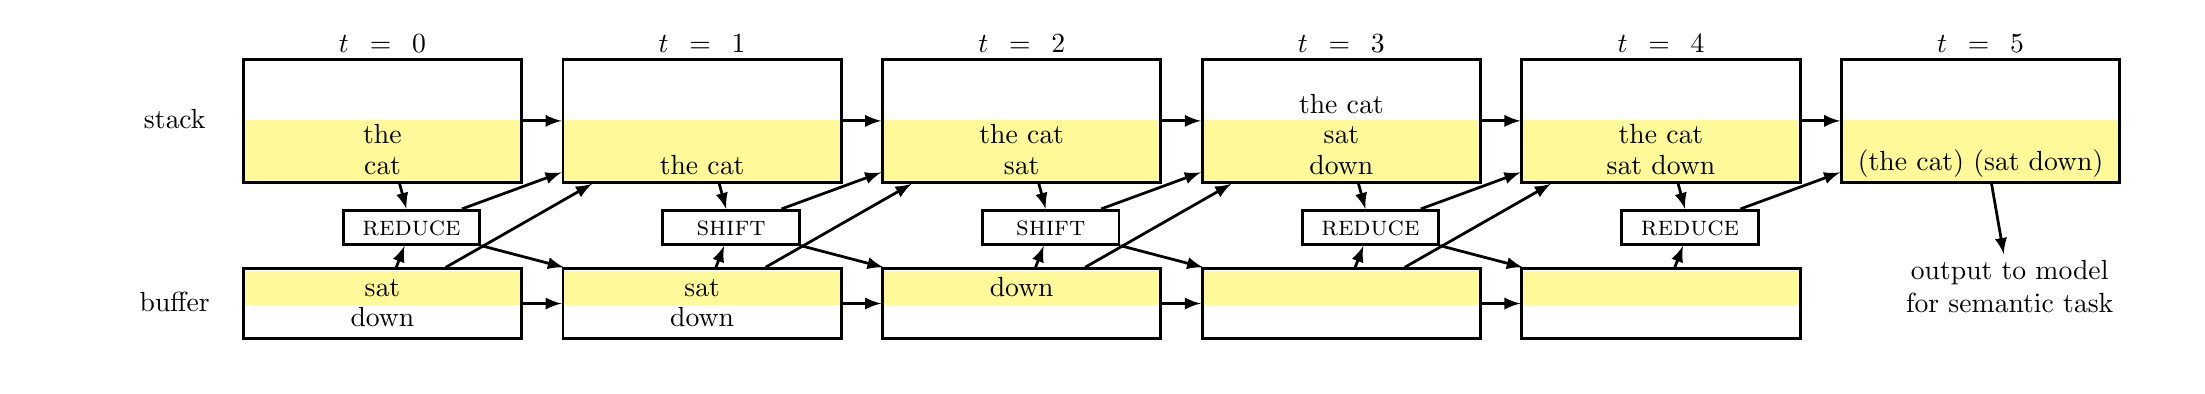
\begin{tikzpicture}
    \def\dx{21pt}
    \def\dy{11pt}
    \def\sy{7*\dy}
    \def\oxb{5.5*\dx}
    \def\by{1*\dy}
    \def\ox{0*\oxb}

    \tikzstyle{label}=[text width=35mm,align=center,text height=2mm]    
    \tikzstyle{word}=[text width=35mm,align=center,text height=2mm]    
    \tikzstyle{tracker}=[fill=red!40,text width=15mm,align=center,text height=2mm]
    \tikzstyle{softmax}=[text width=40mm,align=center,text height=2mm]
    \tikzstyle{comp}=[fill=green!40,text width=20mm,align=center,text height=2mm]
    \tikzstyle{result}=[line width=1pt,draw=black,text width=15mm,align=center,text height=2mm]    
    \tikzstyle{sbox}=[line width=1pt,draw=black,text width=33mm,align=center,text height=13.3mm]
    \tikzstyle{bbox}=[line width=1pt,draw=black,text width=33mm,align=center,text height=6.5mm]
    \tikzstyle{focus1}=[fill=yellow!40,text width=33mm,align=center,text height=2mm]
    \tikzstyle{focus2}=[fill=yellow!40,text width=33mm,align=center,text height=5.5mm]

    \def\ox{0*\oxb}
    
    \node[label]  (1l) at (\ox+0*\dx,\sy+3*\dy) {$t=0$};
    
    \node[label]  (sl) at (\ox-0.65*\oxb+0*\dx,\by+0.5*\dy) {buffer};
    
    \node[focus1] (1bb) at  (\ox+0*\dx,2*\dy) {};
    \node[word]  (1b3) at (\ox+0*\dx,\by-1*\dy) {};
    \node[word]  (1b2) at (\ox+0*\dx,\by+0*\dy) {down};
    \node[word]  (1b1) at (\ox+0*\dx,\by+1*\dy) {sat};
    \node[bbox] (1bb) at  (\ox+0*\dx,\by+0.5*\dy) {};
    
    \node[label]  (sl) at (\ox-0.65*\oxb+0*\dx,\sy+0.5*\dy) {stack};
    
    \node[focus2] (1sb) at  (\ox+0*\dx,\sy-0.5*\dy) {};
    \node[word]  (1s1) at (\ox+0*\dx,\sy-1*\dy) {cat};
    \node[word]  (1s2) at (\ox+0*\dx,\sy+0*\dy) {the};
    \node[word]  (1s3) at (\ox+0*\dx,\sy+1*\dy) {};
    \node[sbox] (1sb) at  (\ox+0*\dx,\sy+0.5*\dy) {};
    
    \node[result] (1so) at  (\ox+0.5*\dx,4*\dy) {\reduce};
              
    \def\ox{1*\oxb}
   
    \node[label]  (1l) at (\ox+0*\dx,\sy+3*\dy) {$t=1$};
    
    \node[focus1] (2bb) at  (\ox+0*\dx,2*\dy) {};
    \node[word]  (2b3) at (\ox+0*\dx,\by-1*\dy) {};
    \node[word]  (2b2) at (\ox+0*\dx,\by+0*\dy) {down};
    \node[word]  (2b1) at (\ox+0*\dx,\by+1*\dy) {sat};
    \node[bbox] (2bb) at  (\ox+0*\dx,\by+0.5*\dy) {};
    
    \node[focus2] (2sb) at  (\ox+0*\dx,\sy-0.5*\dy) {};
    \node[word]  (2s1) at (\ox+0*\dx,\sy-1*\dy) {the cat};
    \node[word]  (2s2) at (\ox+0*\dx,\sy+0*\dy) {};
    \node[word]  (2s3) at (\ox+0*\dx,\sy+1*\dy) {};
    \node[sbox] (2sb) at  (\ox+0*\dx,\sy+0.5*\dy) {};
    
    \node[result] (2so) at  (\ox+0.5*\dx,4*\dy) {\shift};
             
    \def\ox{2*\oxb}
    
    \node[label]  (1l) at (\ox+0*\dx,\sy+3*\dy) {$t=2$};
    
    \node[focus1] (3bb) at  (\ox+0*\dx,2*\dy) {};
    \node[word]  (3b3) at (\ox+0*\dx,\by-1*\dy) {};
    \node[word]  (3b2) at (\ox+0*\dx,\by+0*\dy) {};
    \node[word]  (3b1) at (\ox+0*\dx,\by+1*\dy) {down};
    \node[bbox] (3bb) at  (\ox+0*\dx,\by+0.5*\dy) {};
    
    \node[focus2] (3sb) at  (\ox+0*\dx,\sy-0.5*\dy) {};
    \node[word]  (3s1) at (\ox+0*\dx,\sy-1*\dy) {sat};
    \node[word]  (3s2) at (\ox+0*\dx,\sy+0*\dy) {the cat};
    \node[word]  (3s3) at (\ox+0*\dx,\sy+1*\dy) {};
    \node[sbox] (3sb) at  (\ox+0*\dx,\sy+0.5*\dy) {};
    
    \node[result] (3so) at  (\ox+0.5*\dx,4*\dy) {\shift};

    \def\ox{3*\oxb}
    
    \node[label]  (1l) at (\ox+0*\dx,\sy+3*\dy) {$t=3$};
        
    \node[focus1] (4bb) at  (\ox+0*\dx,2*\dy) {};
    \node[word]  (4b3) at (\ox+0*\dx,\by-1*\dy) {};
    \node[word]  (4b2) at (\ox+0*\dx,\by+0*\dy) {};
    \node[word]  (4b1) at (\ox+0*\dx,\by+1*\dy) {};
    \node[bbox] (4bb) at  (\ox+0*\dx,\by+0.5*\dy) {};
    
    \node[focus2] (4sb) at  (\ox+0*\dx,\sy-0.5*\dy) {};
    \node[word]  (4s1) at (\ox+0*\dx,\sy-1*\dy) {down};
    \node[word]  (4s2) at (\ox+0*\dx,\sy+0*\dy) {sat};
    \node[word]  (4s3) at (\ox+0*\dx,\sy+1*\dy) {the cat};
    \node[sbox] (4sb) at  (\ox+0*\dx,\sy+0.5*\dy) {};
    
    \node[result] (4so) at  (\ox+0.5*\dx,4*\dy) {\reduce};
                  
    \def\ox{4*\oxb}
    
    \node[label]  (1l) at (\ox+0*\dx,\sy+3*\dy) {$t=4$};
    
    \node[focus1] (5bb) at  (\ox+0*\dx,2*\dy) {};
    \node[word]  (5b3) at (\ox+0*\dx,\by-1*\dy) {};
    \node[word]  (5b2) at (\ox+0*\dx,\by+0*\dy) {};
    \node[word]  (5b1) at (\ox+0*\dx,\by+1*\dy) {};
    \node[bbox] (5bb) at  (\ox+0*\dx,\by+0.5*\dy) {};
    
    \node[focus2] (5sb) at  (\ox+0*\dx,\sy-0.5*\dy) {};
    \node[word]  (5s1) at (\ox+0*\dx,\sy-1*\dy) {sat down};
    \node[word]  (5s2) at (\ox+0*\dx,\sy+0*\dy) {the cat};
    \node[word]  (5s3) at (\ox+0*\dx,\sy+1*\dy) {};
    \node[sbox] (5sb) at  (\ox+0*\dx,\sy+0.5*\dy) {};
    
    \node[result] (5so) at  (\ox+0.5*\dx,4*\dy) {\reduce};
    
    \def\ox{5*\oxb}

    \node[label]  (1l) at (\ox+0*\dx,\sy+3*\dy) {$t=5$};

    \node[focus2] (6sb) at  (\ox+0*\dx,\sy-0.5*\dy) {};
    \node[word]  (6s1) at (\ox+0*\dx,\sy-1*\dy) {(the cat) (sat down)};
    \node[word]  (6s2) at (\ox+0*\dx,\sy+0*\dy) {};
    \node[word]  (6s3) at (\ox+0*\dx,\sy+1*\dy) {};
    \node[sbox] (6sb) at  (\ox+0*\dx,\sy+0.5*\dy) {};

    \node[softmax] (6sm) at  (\ox+0.5*\dx,2*\dy) {output to model for semantic task};
                   
    \pgfsetarrowsend{latex}
    \tikzstyle{fwd} = [draw=black, line width=1pt]

   \draw [fwd] (1sb) -- (1so);
   \draw [fwd] (1bb) -- (1so);

    \draw [fwd] (1sb) -- (2sb);
    \draw [fwd] (1bb) -- (2bb);
    \draw [fwd] (1so) -- (2sb);
    \draw [fwd] (1so) -- (2bb);
    \draw [fwd] (1bb) -- (2sb);

   \draw [fwd] (2sb) -- (2so);
   \draw [fwd] (2bb) -- (2so);

    \draw [fwd] (2sb) -- (3sb);
    \draw [fwd] (2bb) -- (3bb);
    \draw [fwd] (2so) -- (3sb);
    \draw [fwd] (2so) -- (3bb);
    \draw [fwd] (2bb) -- (3sb);

   \draw [fwd] (3sb) -- (3so);
   \draw [fwd] (3bb) -- (3so);

    \draw [fwd] (3sb) -- (4sb);
    \draw [fwd] (3bb) -- (4bb);
    \draw [fwd] (3so) -- (4sb);
    \draw [fwd] (3so) -- (4bb);
    \draw [fwd] (3bb) -- (4sb);

   \draw [fwd] (4sb) -- (4so);
   \draw [fwd] (4bb) -- (4so);

    \draw [fwd] (4sb) -- (5sb);
    \draw [fwd] (4bb) -- (5bb);
    \draw [fwd] (4so) -- (5sb);
    \draw [fwd] (4so) -- (5bb);
    \draw [fwd] (4bb) -- (5sb);

   \draw [fwd] (5sb) -- (5so);
   \draw [fwd] (5bb) -- (5so);

    \draw [fwd] (5sb) -- (6sb);
    \draw [fwd] (5so) -- (6sb);

   \draw [fwd] (6sb) -- (6sm);

  \end{tikzpicture}}
  
 \caption{The fully unrolled model for \word{the cat sat down} with some layers omitted for clarity.}\label{fig:model:1b}  
\end{subfigure}
\caption{\label{m1-views}Two views of the transition-based sentence model. In both views, the lower boxes represent the input buffer, and the upper boxes represent the stack. Yellow highlighting indicates which portions of these data structures are visible to the tracking LSTM and to the composition function. Thin gray arrows indicate connections which are blocked by a gating function, and so contribute no information. \todo{[SB] Clean up the arrangements of these figures now that we aren't reporting on Models 1/2.}}
\end{figure*}


\paragraph{The buffer and word representations}

We draw our word representations from the standard 300-dimensional vector package provided with GloVe \cite{pennington2014glove}. We do not update these vectors during training. Instead, we use a learned linear transformation to transform the representation of each input word $\vec{x}$ into a pair of vectors that can be used as inputs to a TreeLSTM composition function:

\begin{equation}
\colvec{2}
    {\vec{h}}
    {\vec{c}}
= W_{\text{wd}} \vec{x}
\end{equation}


\paragraph{The representations in the stack}

In a PINN, each row of the stack contains a pair of vectors $(h, c)$, which together represent some node in the parse tree of the sentence. Since the \shift~operation simply copies entries from the buffer onto the stack, this means that the word representations in the buffer also have two parts, $h$ and $c$. 

\paragraph{The composition function}
When a \reduce~operation is performed, vector representations of two tree nodes are popped off of the head of the stack and fed into a {\ii composition function}, which is a neural network function that produces a representation for a new tree node that is the parent of the two popped nodes. This new node is then pushed on to the stack.

Our composition function is based closely on the TreeLSTM of \citealt{tai2015improved}. The TreeLSTM generalizes the LSTM neural network layer \cite{hochreiter1997long} to tree- rather than sequence-based inputs, and it shares with that older design the idea of representing intermediate states in a computation using a two-part vector representation containing an $\vec{h}$ vector and a $\vec{c}$ vector, where the latter is meant to serve as a slower-changing long-term memory. 

The precise formulation that we use is as follows.

\begin{gather}
\colvec{4}
    {\vec{i}}
    {\vec{f}_l}
    {\vec{f}_r}
    {\vec{o}}
= \sigma(
W_{\text{iffo}}
\colvec{3}
    {\vec{h}_s^1}
    {\vec{h}_s^2}
    {\vec{e}}
)
\\
\vec{g}
= \tanh(
W_{g}
\colvec{3}
    {\vec{h}_s^1}
    {\vec{h}_s^2}
    {\vec{e}}
)
\\
\vec{c} = \vec{f}_l * \vec{c}_s^2 + \vec{f}_r * \vec{c}_s^1 + \vec{i} * \vec{g}  
\\
\vec{h} = \vec{o} * \vec{c}
\end{gather}

The results of this function are the pair $(\vec{h}, \vec{c})$, which are placed back on the stack. The two input tree nodes popped off the stack are represented as the pairs $(\vec{h}^1_s, \vec{c}^1_s)$ and $(\vec{h}^2_s, \vec{c}^2_s)$. In addition, $\vec{e}$ is an optional input argument which is either the empty vector $[]$ or a vector from an external source like the tracking LSTM (see below). $*$ denotes the elementwise product. Each vector-valued variable listed here is of dimension $D$, except $\vec{e}$, which is of dimensions $D_t$, which can be chosen independently.

\paragraph{Creating a sentence pair classifier}

This paper presents the transition-based sentence model within the context of \textit{natural language inference} (also known as \textit{recognizing textual entailment}), a sentence pair classification task. To classify a sentence pair, a feature vector is first constructed. This feature vector is based on the final representations of each of the two sentences---the representations that appear at the head of the stack for each sentence after the final transition. In particular, the $\vec{h}$ portions of these representations are used. The final feature vector consists of the concatenation of these two vectors, $\vec{x}_{\text{premise}}$ and $\vec{x}_{\text{hypothesis}}$, their difference, and their elementwise product:

\begin{equation}
\vec{x}_{classifier} = 
\colvec{4}
    {\vec{h}_{\text{premise}}}
    {\vec{h}_{\text{hypothesis}}}
    {\vec{h}_{\text{premise}} - \vec{h}_{\text{hypothesis}}}
    {\vec{h}_{\text{premise}} * \vec{h}_{\text{hypothesis}}}
\end{equation}

This feature vector is then passed to a series of two (\todo{Update w/ final number}) ReLU neural network layers, then passed into a linear transformation, and then finally passed to a softmax layer, which yields a distribution among the three labels.

\subsection{Tracking left context with an auxiliary LSTM}

Lexical ambiguity is omnipresent in natural language. Most words have multiple senses or meanings, and it is generally necessary to use the context in which a word occurs to determine which of its senses or meanings is meant in a given sentence. Simpler sequence-based sentence encoding models like the standard LSTM RNN have an advantage here: when a sequence-based model first processes a word (first incorporates it into a partial sentence representation), the model has access to a state vector that summarizes all of the words to the left of the current word, and that state vector can serve as a crude but effective form of context to help with disambiguation. In contrast, when standard tree-structured models first process a word, they only have access to the constituent that the word is merging with, which is strictly less than the sequence model has access to, and is often just a single additional word. 

In addition to our basic model, we additionally propose an extension that adds to the model (and exploits its sequential structure) by building in a parallel sequence-based model to track left context. This auxiliary model, called the tracking LSTM, maintains a low dimensional representation that is updated after every transition, thereby maintaining a representation of the left context at each time point. That representation is fed into the composition function as an additional input to allow for more efficient disambiguation. As long as the representations produced by the tracking LSTM are substantially smaller than those produced by the main composition function, the model is heavily biased towards computing sentence meaning compositionally according to the assigned tree structure, and is simply given the ability to do so with a better awareness of context.

The tracking LSTM is a standard LSTM RNN. At each step it takes three vectors as inputs: the top element of the buffer $\vec{h}_b^1$, which would be moved in a \shift~operation, and the two two elements of the stack $\vec{h}_s^1$ and $\vec{h}_s^2$ which would be composed in a \reduce~operation. Its output hidden state at each step is used as the external input to the TreeLSTM composition function for that step.

\subsection{Parsing: Predicting transitions from the tracking state}

\todo{[SB] Fill in math, Explain.}

\subsection{Implementing the transition-based sentence model}

\paragraph{The size of the stack}
The size of the stack should be $N$ for sentences of $N$ words, in case the first reduce merges the final two words. The size of the buffer should be $N$.

\paragraph{Converting parses to transition sequences}

For Models 0--3, all training data must be parsed in advance into an unlabeled binary constituency tree. In addition, Model 0 requires that  parses be available at test time as well. For both SST and SNLI we use the parses included with the corpus distributions whenever parses are needed. 

For model 0, training data can be prepared by linearizing the provided parse, then deleting left brackets and replacing right brackets with \reduce~instructions. That is demonstrated here with the example sentence \ii{the cat sat down}:

\begin{quote}\small
( ( the cat ) ( sat down ) )$\Rightarrow$\\
the cat \reduce~sat down \reduce~\reduce
\end{quote}

The input for models 1--4 is simply the word sequence from the parse, with the first two words moved into the stack. The syntactic supervision labels for models 1--3 are simply a binarized version of the Model 0 inputs, with the first two tokens (which are necessarily \shift~\shift) omitted: 

\begin{quote}\small
( ( the cat ) ( sat down ) )$\Rightarrow$ \\
stack: $\langle$the, cat$\rangle$\\
buffer: $\langle$sat, down$\rangle$\\
ops: \reduce~\shift~\shift~\reduce~\reduce
\end{quote}

\paragraph{Handling variable sentence lengths}

To efficiently implement batched computation, we must stipulate a fixed number of transitions (50) that the model can perform before producing an output. Sentences whose transition sequences are shorter than this length are padded, and sentences whose transition sequences are longer than this length are cropped. 

Padding, if done properly, should not impact the output of the model significantly:\footnote{The tracking LSTM can cause a slight dependence of the final representation on unrolling length. Because of this, we always train and test the model with a fixed unrolling length.} a model with the fixed parameters should produce the same representation for a 10-word sentence whether it is unrolled for 19 transitions (the minimum to avoid cropping) or 100.

Cropping necessarily discards information, but if done properly, it is nonetheless possible to learn good representations for cropped sentences. When a transition sequence is cropped, the number of removed \shift~transitions is tracked, and an equal number of word tokens is removed from the tail (left) end of the buffer. This makes it possible for a transition sequence to begin with a \reduce~transition, or to otherwise use a \reduce~transition on a stack that does not have two elements to reduce. In this instance, we simply feed the composition function one or more zero vectors, which represent nonexistent stack elements. If the composition learns to interpret these zero vectors properly, they can be taken to be unknown or incomplete nodes in an otherwise complete tree that is constructed according to the intended parse structure. \todo{[SB] Make a figure showing the results of cropping if there's room.}

\paragraph{Representing the stack in memory} Or, thin stack. And the cursor strategy for the buffer. 
\todo{[JG] Explain.}

\vspace{8em}

\paragraph{Optimization and hyperparameters}

We use the RMSProp optimizer (\todo{Cite.}) with a tuned starting learning rate that decays by a factor of 0.75 every 10k steps. We apply both dropout \cite{srivastava2014dropout} and batch normalization \cite{2015SIoffeCSzegedy} to the word embeddings in the buffer (after the linear projection is applied) and to the feature vectors that serve as the inputs and outputs to the MLP that precedes the final entailment classifier. In addition, we apply an L2 regularization penalty to all parameters.

We used random search to tune many of the hyperparameters, including the learning rate, the dropout rate, the L2 regularization weight, the hidden dimension of the tracking LSTM and the number of layers in the MLP \todo{[SB] Report the ranges searched for each parameter and the number of runs for each results.}

We trained each model for 250k steps in each run, using a minibatch size of 64 for each step. We tracked each model's performance on the development set during training and saving parameters when this performance reached a new peak. We used early stopping, evaluating on the test set using the parameters that performed best on the development set.

\paragraph{Software infrastructure} We will make Theano code available.

\subsection{TreeRNN-equivalence and efficiency}

In its bare form, before the addition of the tracking LSTM, the PINN computes the precisely the same functions as a conventional tree-structured neural network model, and has the same learning dynamics: the representation of each sentence consists of the representation of the words, combined recursively using a TreeRNN composition function (in our case, the TreeLSTM function). While it adds no expressive power on its own, this design improves upon the standard TreeRNN implementation in three ways:

\begin{itemize}
\item It provides a straightforward strategy for implementing tree-structured composition which allows for batched computation, and provides near-optimal run times on typical computer systems. While our design includes some wasted computation induced by the full application of the composition function at every step, this is made up for by avoiding most of the (potentially expensive) scattered memory access that would be needed for batched computation strategies that more closely mimic the standard tree-based architecture.

\item It provides a simple mechanism for integrating the use of left-context into tree-structured models through the tracking LSTM, providing a fast mechanism to help these models handle lexical ambiguity.

\item By designing the model around the standard transition set used in neural network syntactic parsers, it opens the door to tight integration between parsing and sentence interpretation, including the possibility of joint learning, or even of learning a parser trained entirely on a sentence classification or interpretation objective.
\end{itemize}

\subsection{Related work: Transition-based parsing and neural networks.}

There has been a fairly long history of work on building neural-network based parsers that use the core operations and data structures from transition-based parsing \cite{henderson2004discriminative,emami2005neural,titov2010latent,buys2generative,chen2014,dyer-EtAl:2015:ACL-IJCNLP,kiperwasser2016easy}. In addition, there has been recent work \cite{zhang2016top,dyer2016rnn} proposing models designed primarily for generative language modeling tasks that use these structures as well. To our knowledge, the PINN is the first model to use these structures for the purpose of sentence interpretation, rather than parsing or generation.

\section{Attention over trees}

%!TEX root = gist.tex

\begin{figure*}[t]
\centering
\scalebox{0.8}{
 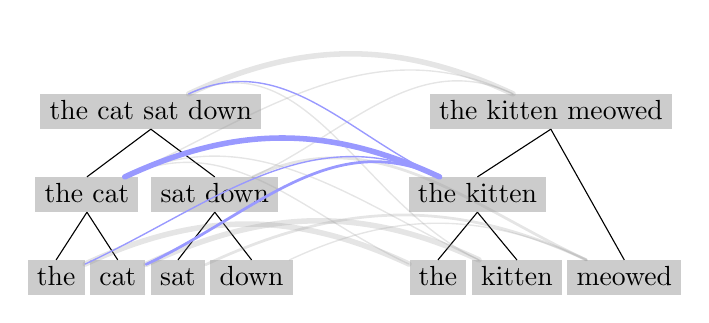
\begin{tikzpicture}
    \tikzstyle{word}=[fill=black!20,text height=2mm]    
    \tikzstyle{nonleaf}=[fill=black!20,text height=2mm]    

    \begin{scope}[shift={(0in,0in)}, frontier/.style={distance from root=60pt}]

    \Tree [.\node[nonleaf](1thecatsatdown){the cat sat down}; [.\node[nonleaf](1thecat){the cat}; \node[word](1the){the}; \node[word](1cat){cat}; ] [.\node[nonleaf](1satdown){sat down}; \node[word](1sat){sat}; \node[word](1down){down}; ] ]

    \end{scope}

    \begin{scope}[shift={(2in,0in)}, frontier/.style={distance from root=60pt}]

    \Tree [.\node[nonleaf](2thekittenmeowed){the kitten meowed}; [.\node[nonleaf](2thekitten){the kitten}; \node[word](2the){the}; \node[word](2kitten){kitten}; ] \node[word](2meowed){meowed}; ]

    \end{scope}
    
    \usetikzlibrary{arrows,scopes}

    \tikzstyle{attn} = [line width=1pt,draw=black!40,opacity=0.25,line cap=round]
    \tikzstyle{heavy} = [line width=2pt]
    \tikzstyle{light} = [line width=0.5pt]
    \tikzstyle{focus} = [draw=blue!40,opacity=1.0]

    \draw [attn,heavy] (1the) to[in=155,out=25] (2the);
    \draw [attn,light] (1thecat) to[in=155,out=25] (2the);

    \draw [attn,heavy] (1cat) to[in=155,out=25] (2kitten);
    \draw [attn,light] (1thecat) to[in=155,out=25] (2kitten);
    \draw [attn,light] (1thecatsatdown) to[in=155,out=25] (2kitten);

    \draw [attn,light] (1satdown) to[in=155,out=25] (2thekittenmeowed);
    \draw [attn,light] (1thecat) to[in=155,out=25] (2thekittenmeowed);
    \draw [attn,heavy] (1thecatsatdown) to[in=155,out=25] (2thekittenmeowed);

    \draw [attn] (1satdown) to[in=155,out=25] (2meowed);
    \draw [attn] (1sat) to[in=155,out=25] (2meowed);
    \draw [attn,light] (1down) to[in=155,out=25] (2meowed);

    \draw [attn,focus] (1cat) to[in=155,out=25,] (2thekitten);
    \draw [attn,heavy,focus] (1thecat) to[in=155,out=25] (2thekitten);
    \draw [attn,light,focus] (1the) to[in=155,out=25] (2thekitten);
    \draw [attn,light,focus] (1thecatsatdown) to[in=155,out=25] (2thekitten);

  \end{tikzpicture}}
  
 \caption{Soft alignments between the nodes of two trees, with alignments to ``the kitten'' highlighted in blue.}\label{fig:tree_attn}
\end{figure*}


\paragraph{Constituent-by-constituent attention}
We aim to build on the results of \citealt{rocktaschel2015reasoning} and \citealt{wang2015learning}, who find that neural soft attention models is an extremely effective technique for learning natural language inference. In particular, both papers use versions of word-by-word entailment, in which a latent alignment is learned from every word in the hypothesis to one or more words of the premise. We propose to borrow this basic idea, but to adapt it to a tree-structured setting, proposing \textit{constituent-by-constituent} attention. While these models do attention over a matrix $\mathbf{Y}$ of word-in-context representations from the premise encoder, we will perform attention instead over our own primary data structure, $\mathbf{Y}^{st}$, the matrix of vectors that have appeared at the top of the stack during premise encoding, which correspond one-to-one to the constituents in the tree structure representing the premise. Similarly, while the previous models perform one instance of soft attention conditioned on each word in the hypothesis, we perform one instance of soft attention conditioned on each stack top in the hypothesis encoder, representing the constituents of the hypothesis tree.

In the PINN, attention is performed at each step $t$ of the premise encoder. At step $t$, the query vector that drives attention will be $S^t_0$, the top of the stack. 

\todo{[AR, RG] Write up the attention equations that you use.}

\subsection{Accumulating the results of attention}

\todo{[RG,AR] Accumulating results sequentially  (After Rocktäschel, Wang and Jiang)}

\todo{[RG,SB] Accumulating results using a second tree layer}

\section{Experiments}

\subsection{Natural language inference and SNLI}

We evaluate the PINN on the task of natural language inference (NLI), also known as recognizing textual entailment (RTE). NLI is a sentence pair classification task, in which a model reads two sentences (a premise and a hypothesis), and outputs a judgment of {\it entailment}, {\it contradiction}, or {\it neutral}, reflecting the relationship between the meanings of the two sentences, as in this example from the Stanford NLI corpus (SNLI, \citealt{snli:emnlp2015}), which we use for training and evaluation: 

\begin{quote}
Premise: {\it Girl in a red coat, blue head wrap and jeans is making a snow angel.}

Hypothesis: {\it A girl outside plays in the snow.}

Correct label: {\it entailment}
\end{quote}

Even though NLI is framed as a relatively simple three-way classification task, it is nonetheless an effective way of evaluating the ability of some model to extract broadly informative representations of sentence meaning. In order for a model to reliably perform well on NLI across a range of sentence types and text genres, it must be able to represent and reason with all of the core phenomena of natural language semantics, including quantification, coreference, scope, and several types of ambiguity.

SNLI is a corpus of 570k human-labeled pairs of scene descriptions like the one above. We use the standard train--test split and ignore unlabeled examples, which leaves about 549k examples for training, 9,842 for development, and 9,824 for testing. SNLI labels are roughly balanced, with the most frequent label, {\it entailment}, making up 34.2\% of the test set.

\subsection{Models evaluated}

We evaluate five models on the SNLI task. Each uses 300d hidden states: \todo{[SB] Reframe around M1.}
\begin{itemize}
\item A baseline LSTM model (similar to that of \citealt{snli:emnlp2015}) that uses the same classifier architecture as our models, but encodes sentences using a single layer LSTM RNN sequence model.
\item The unaugmented transition-based sentence model.
\item The transition-based sentence model with the tracking LSTM.
\item The transition-based sentence model with the tracking LSTM and sequence-based attention over premise states.
\item The transition-based sentence model with the tracking LSTM and tree-based attention over premise states.
\end{itemize}

\begin{table*}[t]
  \centering\small
  \begin{tabular}{lcccc} 
    \toprule
Model                   & Params.    & Trans. acc.  &   Train  &   Test \\
\midrule
\multicolumn{4}{c}{Previous non-NN results}\\
\midrule
Lexicalized classifier \cite{snli:emnlp2015}
                        & --                & --                    &   99.7   &   78.2      \\
\midrule
\multicolumn{4}{c}{Previous NN results without attention}\\
\midrule
100d LSTM encoders \cite{snli:emnlp2015}
                        & 221k               & --               &   84.8   &   77.6      \\
1024d pretrained GRU encoders \cite{DBLP:journals/corr/VendrovKFU15}
                        & 15m                & --              &   98.8   &   81.4       \\
300d Tree-based CNN encoders \cite{mou2015recognizing}
                        & 3.5m                & --             &   83.4   &   82.1       \\
\midrule
\multicolumn{4}{c}{Previous NN results with attention}\\
\midrule
100d LSTM w/ word-by-word attention \cite{rocktaschel2015reasoning}
                        & 252k               & --              &   85.3   &   83.5       \\
300d mLSTM word-by-word attention model \cite{DBLP:journals/corr/WangJ15b}
                        & 1.9m               & --             &   92.0   &   86.1      \\
300d LSTMN with deep attention fusion \cite{cheng2016long}
                        & 1.4m               & --                &   92.3   &   89.1      \\
\midrule
\multicolumn{4}{c}{New results}\\
\midrule
\result{300d LSTM RNN      } & ?             & --                &   ?      &   81?       \\
\result{300d PINN-GT w/o tracking}   
                        & ?                  & --                &   ?      &   81?       \\
\result{300d PINN-GT }
                        & ?                  & --                &   ?      &   83?       \\
\result{300d PINN }
                        & ?                  & ??                  &   ?      &   83?       \\                        
\result{300d PINN-GT, sequence-based attn.   }     
                        & ?                  & --                &   ?      &   85+?       \\
\result{300d PINN-GT, tree-based attn. }           
                        & ?                  & --                &   ?      &   \textbf{?}\\
    \bottomrule
  \end{tabular}
  \protect\caption{\protect\label{tab:results}Results on SNLI 3-way inference classification. Params. is the approximate number of trained parameters (excluding word embeddings for models where they are trained). Trans. acc. is the model's accuracy in predicting parsing transitions. Train and test are SNLI classification accuracy. \result{[JG]Add seconds-per-step *if* we get a reasonably well-optimized model in time.}} 
\end{table*}

\paragraph{Results}

Table~\ref{tab:results} shows our results.

\subsection{Step time}

\todo{[JG,SB] Does anyone know of a better baseline TreeRNN implementation that we can use on Jagupard? We can use the CoreNLP SST model, but using a Java model as a baseline seems worrying unless we're guaranteed that it's competitively fast.}

Comparing model step time to the plain RNN of \citealt{li2015tree}. We use the small \citealt{pang2004sentimental} sentiment corpus that they use, and train with identical hyperparameters: ...

\section{Discussion}

\result{Patterns in the examples that the tree model got right that the LSTM didn't}

\result{Induced alignments}

\begin{figure}
\vspace{14em}
\caption{\label{fig:induced-alignment}The alignment induced between two sentences by \result{one of our models.}. Compare with a similar alignment presented by \protect\citealt{DBLP:journals/corr/WangJ15b}.}
\end{figure}

\section{Conclusions and future work}

\begin{itemize}
\item It is possible to train a tree-structured model, without approximation, on large-scale language learning tasks.
\item Tree structure helps in large-scale language learning tasks. Not massively, but measurably.
\item The advantages of attention carry over to tree-structured models.
\end{itemize}

\paragraph{Future work} The tracking LSTM that we incorporated into the PINN uses only simple, quick to compute features drawn from the head of the buffer and the head of the stack. It is plausible that giving the tracking LSTM access to more information from the buffer and stack at each step would allow it to better represent the context of each tree node, including information about that nodes neighbors in the sentence string and its likely position in the final tree, and that that context information could support better sentence encoding. One promising way to pursue this goal would be to encode the full contents of the stack and buffer at each time step following the method used by \citealt{dyer-EtAl:2015:ACL-IJCNLP} for parsing.
The model presented here is only capable of operating over sentences which have already been assigned a binary constituency tree by a parser. This is not necessarily a practical limitation, since modern parsers can assign reasonably high quality parses in so little time as to not dramatically impact the performance characteristics of our model \todo{[SB,JG,CM] How fast are fast constit parsers?}. However, depending upon an external parser can be a missed opportunity.

\todo{[SB] Remove Model 1 references.}

In future work, we aim to incorporate a parser into our model, allowing it to simultaneously learn to parse sentences (using a conventional parsing objective function) and to use those parses to learn semantic representations for those sentences (using a classification objective function, as in this work). Implementing such a model on top of our proposed stack-based design would learn a model that could productively share representations between the two tasks. Implementing such a model on top of a differentiable version of our stack-based design (possibly following \citealt{grefenstette2015learning,joulin2015inferring}) would further make it possible for the model to learn to parse using guidance from the semantic representation objective, essentially allowing  learn to produce parses that are, in aggregate, better suited to supporting semantic interpretation than those supplied in the training data. 

%    \subsubsection*{Acknowledgments}
%    
%    Some of the Tesla K40(s) used for this research was/were donated by the NVIDIA Corporation.
%    \todo{[CM,CP] Acknowledge other grants.}

\bibliographystyle{../acl}
\bibliography{../MLSemantics}
\todo{[SB] Make bibliography style uniform.}

\end{document}
